\chapter{Minimalflächen\label{chapter:thema}}
\lhead{Minimalflächen}
\begin{refsection}
\chapterauthor{Nadja Rutz und Ambroise Suter}

\section{Einleitung}
\rhead{Einleitung}

Flach aber trotzdem krumm!

Schon im Kindesalter lernen wir den Begriff der Krümmung kennen, doch gerade im mehrdimensionalen Raum gestaltet sich die Vorstellung und Berechnung von Krümmung als nicht ganz einfach. 

Die Menschheit brauchte mehrere Jahrtausende um herauszufinden, dass die Erde nicht flach sondern gekrümmt ist. 
Ähnliche Diskussionen kamen auch in der Kosmologie des Universums auf.
Viele Experimente zeigen, dass das Universum Flach ist. 
Je nach intrinsischer (innerer) und extrinsischer (äusser) Krümmung kann ein Raum aber auch flach sein wenn er extrinsisch gekrümmt ist.


\section{Problemstellung}
\rhead{Problemstellung}

Minimalflächen haben eine mittlere Krümmung von Null. 

In diesem Kapitel werden zuerst verschiedene Krümmungsarten von Flächen vorgestellt, um anschliessend den Spezialfall der Minimalflächen genauer betrachten zu können. 
Zur Illustration werden einige Beispiele von Minimalflächen gerechnet. 
Als Vorstellungshilfe dienen oft nicht geschlossene Seifenfilme da diese von Natur aus  Minimalflächen erzeugen.


\subsection{Krümmung einer Fläche}
\index{Krümmung einer Fläche}

Intuitiv ist Krümmung einer Fläche für uns ein Mass der Abweichung eines Objekts im Bezug zu einer flachen Fläche. 

Die Krümmung einer Fläche im Punkt P kann in der Mathematik indirekt durch die Hauptkrümmungsradien $R1$ und $R2$ ausgedrückt werden. 
Die Hauptkrümmungsradien hängen von den Tangentenrichtungen im Punkt P ab. 
Die Tangentenrichtungen stehen senkrecht aufeinander.
Sie sind so definiert, dass $R1$ den Minimalwert und $R2$ den Maximalwert annimmt.

Unter einem Krümmungsradius versteht man den Radius des Kreises welcher die Kurve im Punkt P am besten approximiert. 
Da wir intuitiv bei einem Kreis oder einer Kugel eine grosse Krümmungszahl erwarten und bei einer fast geraden Fläche eine kleine, ist die Krümmung $k$  als der Kehrwert vom Krümmungsradius definiert. $k=1/R$ 

\begin{figure} [H]
  \centering
  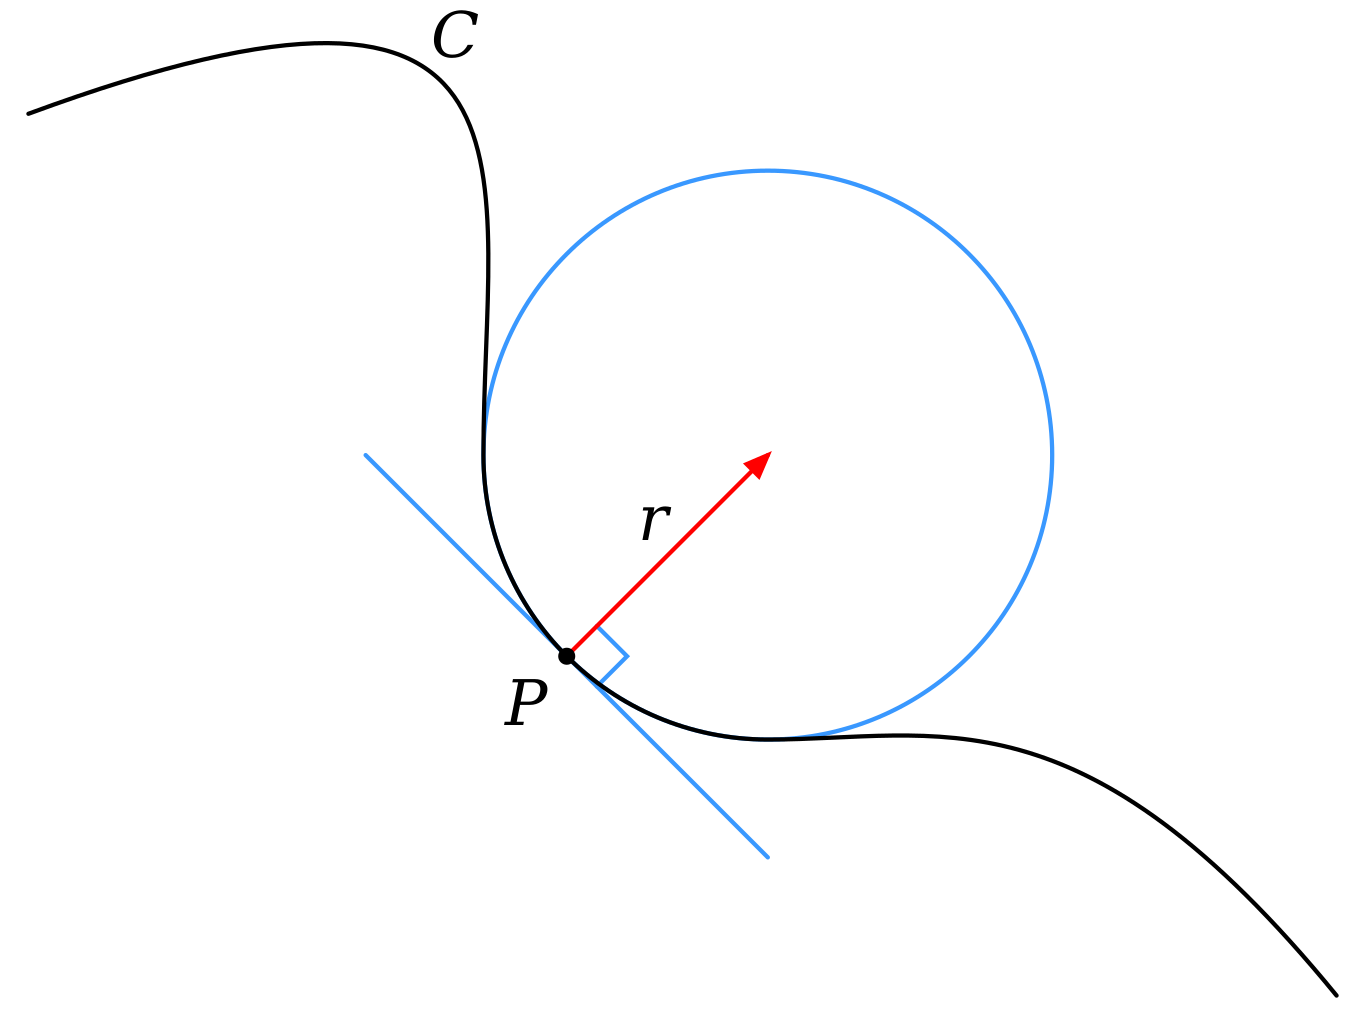
\includegraphics[scale=0.1]{minimal/Kruemmungsradius.png}
  \caption{Krümmungsradius} 
\end{figure}


Zur numerischen Charakterisierung der Krümmung einer Fläche in der Mathematik werden hauptsächlich zwei Grössen benutzt.
Zum einen die Gauss Krümmung was eine intrinsische Krümmung ist und zum andern die Mittlere Krümmung bei welcher es sich um eine extrinsische Krümmung handelt. Bei Minimalflächen ist vor allem die Mittlere Krümmung von Bedeutung, da diese dort null ist.

\index{Gauss Krümmung}

Die Gauss Krümmung einer Fläche im Punkt P ist definiert als das Produkt der zwei Hauptkrümmungen k1 und k2.

\begin{equation} \label{Gauss_Kruemmung_D}
  H=k1\, k2= \frac{1}{R1}\frac{1}{R2}
\end{equation}



Die Gauss Krümmung ist eine intrinsische Krümmung. Diese ist  ein Mass für die innere Krümmung einer Fläche. 
Eine gute Vorstellungshilfe ist die Ameisenperspektive. 
Wenn die Ameise auf einer Kugel ist kann sie feststellen, dass nur schon in ihrem kleinen Blickfeld die Winkelsummen eines Dreiecks auf der Oberfläche grösser als 180° ist, demzufolge besitzt die Kugel eine positive Gauss Krümmung. Anders sieht es aus bei einem Zylinder dort misst die Ameise auf der Zylinderoberfläche genau 180° Winkelsumme, das heisst die Gauss Krümmung eines Zylinders ist null.

\index{Mittlere Krümmung}

Die Mittlere Krümmung einer Fläche im Punkt P ist definiert durch den Mittelwert der zwei Hauptkrümmungen k1 und k2.

\begin{equation} \label{Mittlere Kruemmung_D}
  H=\frac{1}{2}(k1+k2)= \frac{1}{2}\bigg(\frac{1}{R1}+\frac{1}{R2}\bigg)
\end{equation}

Die Mittlere Krümmung ist eine extrinsische Krümmung. 
Im Gegensatz zur intrinsischen Krümmung kommt es bei einer extrinsischen Krümmung auf die Umgebung an. 
Man kann sich vorstellen, dass man zum Beispiel die Krümmung eines Zylinders (zweidimensionales Objekt) von aussen, also in einem dreidimensionalen Raum betrachtet. 
Ein Zylinder ist aus der Ameisenperspektive flach, schaut man von aussen sieht er jedoch gekrümmt aus.
Dies weil er eine positive mittlere Krümmung aufweist. 
Anders sieht es zum Beispiel bei einer Sattelfläche (Pringels-Chips artigen Fläche) dort ist die Gausskrümmung ungleich null, hingegen kann die Mittlere Krümmung im Spezialfall, dass $R1=-R2$ gleich null sein. In diesem Fall ist diese Sattelfläche ein Beispiel für eine Minimalfläche.

\begin{figure} [H]
  \centering
  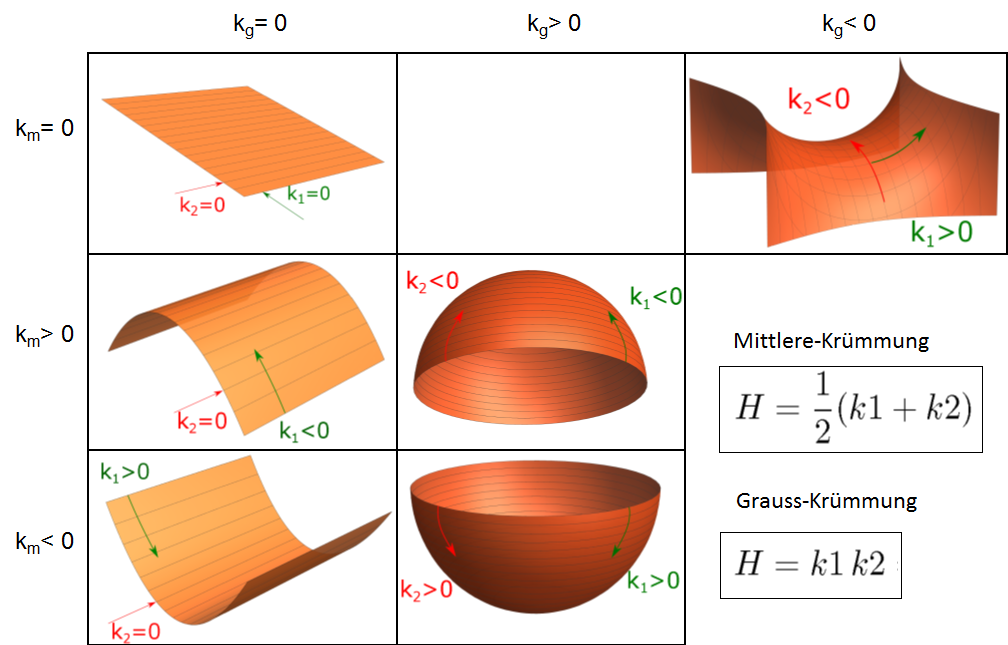
\includegraphics[scale=0.4]{minimal/Tabelle_Kruemmung.png}
  \caption{Vergleich Grauss und Mittlerkrümmung} 
\end{figure}




\section{Defintion der Minimalfläche}
\index{Definition der Minimalfläche}

Um den Begriff der Minimalfläche greifbarer zu gestalten werden hier verschiedene Definitionen, die zueinander gleichwertig sind, erörtert.

\subsection{Variationsproblem}

Def: Eine Fläche $ \textit{M} \subset \mathbf{R}^{3} $ ist genau dann minimal wenn in allen Punkten $p \in M$ die Mittlere Krümmung $=0$ ist.\\
Nach der Definition der Mittleren Krümmung \eqref{Mittlere Kruemmung_D} bedeutet dies, dass in jedem Punkt $p$ sich die Krümmungen $k1$ und $k2$ aufheben.
Folglich entspricht eine Minimalfläche der Geodäte im zwei Dimensionen. Zwei Punkte $P1$ und $P2$ können auf der Fläche über eine kürzeste Strecke verbunden werden.  Dies ist sogleich die erste und in diesem Buch wichtigste Definition der Minimalfläche.

\subsection{Lokale Minimalfläche}

Def: Eine Fläche $ \textit{M} \subset \mathbf{R}^{3} $ ist genau dann minimal wenn alle Punkte $ p \in M $ in der Umgebung  im Verhältnis zum Rand am wenigsten Fläche hat.

In anderen Worten ist eine Fläche minimal wenn deren Teilflächen beliebiger grösse ebenfalls minimal sind.  

\subsection{Seifenfilm}

Def: Eine Fläche $ \textit{M} \subset \mathbf{R}^{3} $ ist genau dann minimal wenn jeder Punkt $p \in M$ eine Umgebung mit Rand $D_p$ gleich dem idealem Rand eines Seifenfilms $\partial D_p$ hat.

In diesem Fall ist die Krümmung eines Seifenfilms proportional zum Druckunterschied auf beiden Seiten der Fläche. Die unterschiedlichen Drücke verformen dabei den Film bis auf beiden Seiten der gleiche Druck vorherrscht. Dies kann beispielsweise mit Seife auf einem Drahtgeflecht visualisiert werden. Seifen\textit{blasen} sind nach dieser Definition keine MF, da sie zum Erhalt ihrer Form einen höheren Innendruck haben.

\begin{figure}[H]
  \centering
  \includegraphics[scale=0.3]{minimal/SattelflacheSoapFilm.png}
  \caption{Seifenfilm bildet Minimalfläche} 
\end{figure}

\subsection{Energie}
Def: Eine Fläche $M \subset \mathbf{R}^{3}$ ist genau dann minimal wenn jeder Punkt $p \in M$ eine Umgebung mit minimaler Energie hat.\\
Äquivalent wie die Kettenlinie, welche die Kräfte zwischen den Kettengliedern minimiert, minimiert eine Minimalfläche die "Spannungen" zwischen den Punkten. Stellt man sich die Fläche als dünne Kautschuk-Haut vor, sieht man schnell, dass die einzelnen Kohlenstoff-Ketten die Kräfte innerhalb des Materials ausgleichen und gleichmässig aufteilen. Dies geschieht insbesondere durch die Van der Waals Kräfte zwischen den Kohlenstoff-Ketten.

\begin{figure}[H]
  \centering
  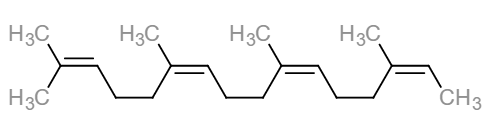
\includegraphics[scale=0.7]{minimal/cis-Polyisopren.PNG}
  \caption{Kohlenstoffkette von Naturkautschuk} 
\end{figure}


\section{Beispiele}
\index{Beispiele}
\subsection{Katenoid}
Wen man zwei drahtringe parallel zueinander in Seifenwasser taucht entsteht die Form eines Katenoids. 
\begin{figure}[H]
  \centering
  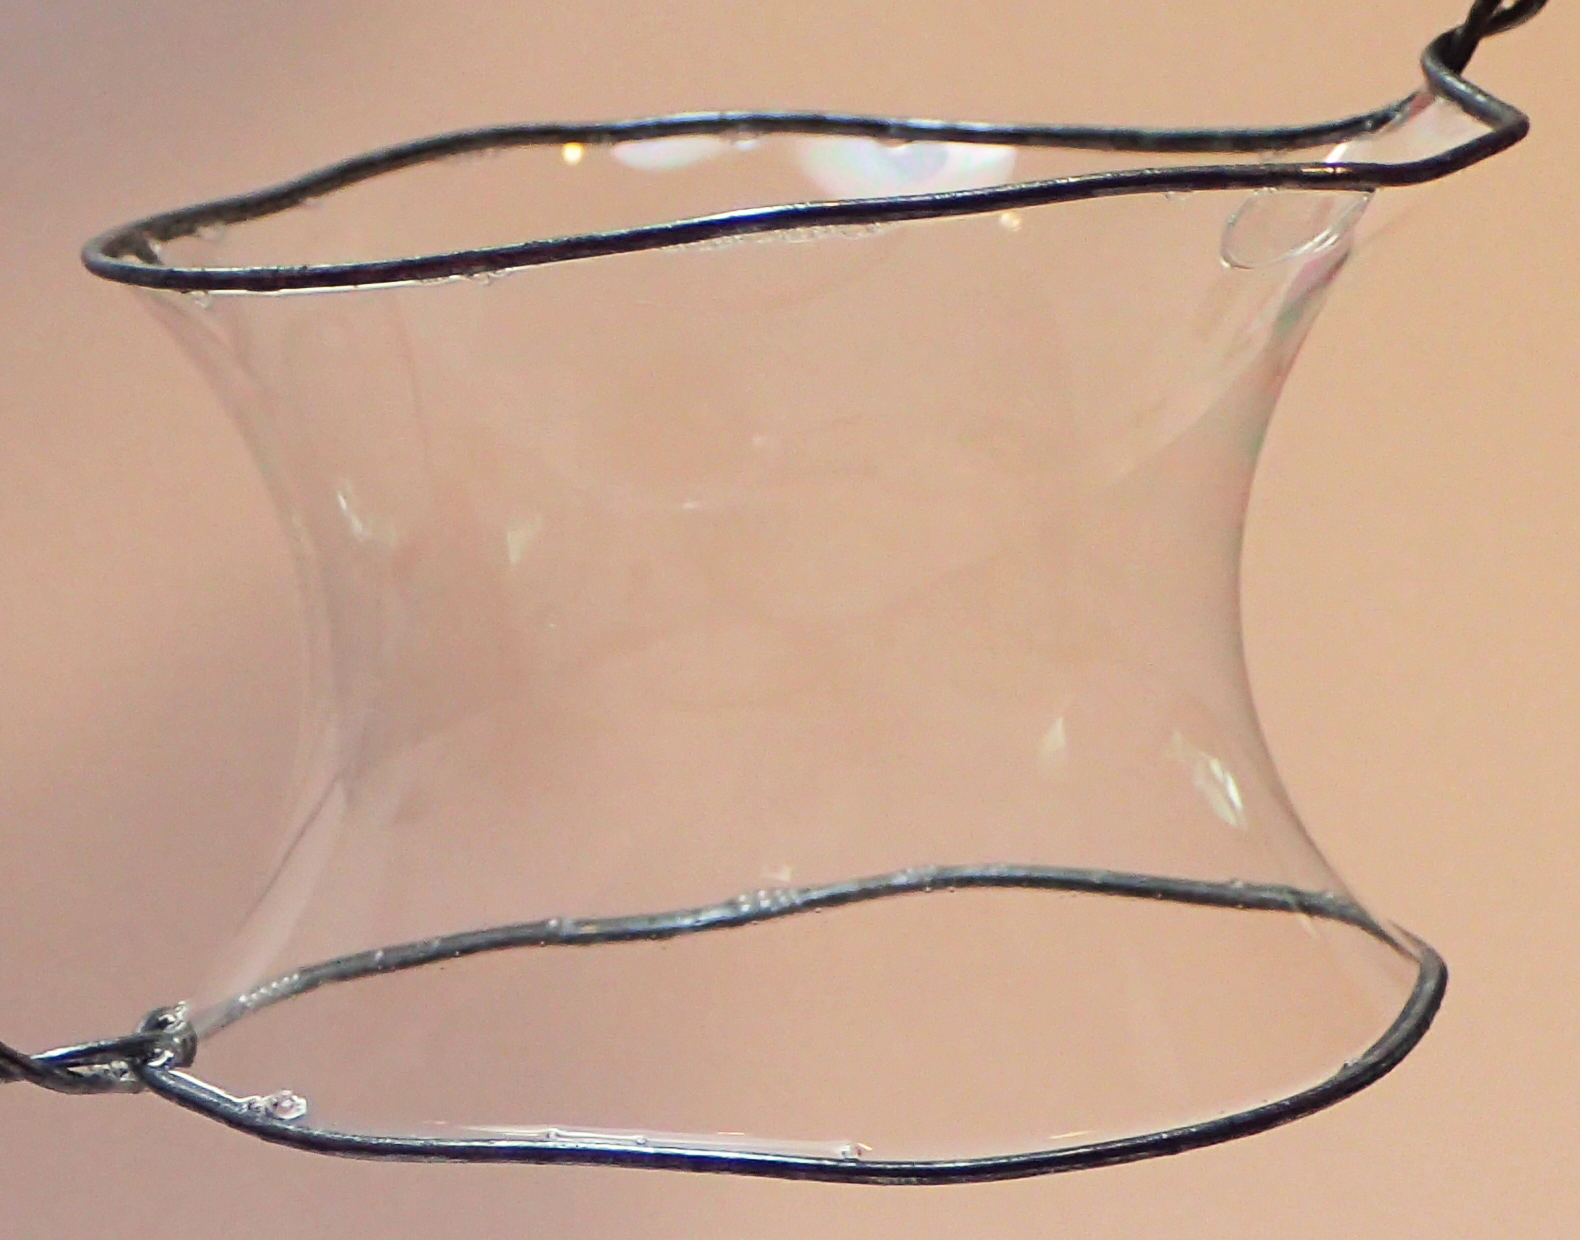
\includegraphics[scale=0.5]{minimal/Cartenoid_Foto.png}
  \caption{Skizze: Seifenfilm-Katenoid} 
\end{figure}
Das Katenoid ist die als erstes entdeckte Minimalfläche.
Sie würde schon 1776 von Herr Jean Baptiste Meusnier erstmals beschrieben.
In diesem Abschnitt wird die mathematische Berechnung des Katenoids mithilfe der Eulerschen Differenzialgleichung der Variationsrechnung beschrieben.
\begin{figure}[H]
  \centering
  \includegraphics[scale=0.3]{minimal/Catenoid3-4Mark}
  \caption{Skizze: Katenoid} 
\end{figure}
In obiger Skizze ist ein Katenoid abgebildet bei welchem in Bezug auf sie $z$ Achse, der untere Drahtring bei $-L$ und der obere bei $+L$ ist. 
Die beiden Kreise sollen die gleichen Radien haben also gilt $r(-L)=r(+L)=R$. Die flächenpunkte des Katenoids werden mit der Funktion $r(z)$ beschrieben. 
Um die Fläche des Katenoids zu berechnen, braucht man eine Gleichung welche eine länge auf der Katenoidoberfläche beschreibt. Mit Hilfe von Pythagoras kann man schreiben $ds^2=dz^2+dr^2$.
Formt man diese Gleichung um erhält man die Gleichung \eqref{ds}.

\begin{equation} \label{ds}
  ds=\sqrt{dz^2\bigg(1+\frac{dr^2}{dz^2}\bigg)}= \sqrt{dz^2(1+\dot r^2)}=\sqrt{(1+\dot r^2)}\,dz
\end{equation}
\subsubsection{Minimalfläche}
Der Seifenfilm versucht automatisch sich im minimalenergetischen Zustand zu befinden. In diesem Zustand ist dann auch die Fläche $S$ des Seifenfilms minimal.
Demzufolge muss das integral \eqref{S1} minimiert werden. 
\begin{equation} \label{S1}  
  S= \int 2 \pi r ds 
\end{equation}
Durch einsetzen von Gleichung \eqref{ds} erhält man die Gleichung \eqref{S2}, welche man als Funktion $F(r,\dot r, z)$ noch verallgemeinert schreiben kann.
\begin{equation} \label{S2}
  S=2 \pi \int_{-L}^{+L} r\sqrt{(1+\dot r^2)}\,dz =2 \pi \int_{-L}^{+L}  F(r,\dot r, z) \,dz 
\end{equation}


Um dieses Integral \eqref{S2} zu minimieren kann man sich der Eulerschen Differenzialgleichung der Variationsrechnung bedienen. 
\subsubsection{Variationsrechnung}
Die Eulerschen Differenzialgleichung der Variationsrechnung wird im Kapitel der Geodäten genauer erklährt.
Das Anwendungsprinzip kurz zusammengefast ist, hat man ein kompliziertes Integral welches man nicht einfach fundamental lösen kann um die Extremwerte zu bestimmen kann man die Eulersche DGL anwenden. Diese besagt, dass anstelle des Ausrechnens eines einer Integralfunktion der Art \eqref{E_DGL1} kann auch die DGL \eqref{E_DGL2} gelöst werden um die Extremwerte solcher Funktionen zu finden.

\begin{equation} \label{E_DGL1}  
  I(y)= \int_a^b F(x,y(x),\dot y(x))\,dx       
\end{equation}

\begin{equation} \label{E_DGL2}
\bigg(\frac{\partial F}{\partial y}\bigg)- \frac{d}{dx} \bigg(\frac{\partial F}{\partial \dot{y}}\bigg)=0         
\end{equation}

Für die Gleichung des Katenoids \eqref{S2} erhält man somit die DGL \eqref{K_DGL1}.
\begin{equation} \label{K_DGL1}
\bigg(\frac{\partial F}{\partial r}\bigg)- \frac{d}{dz} \bigg(\frac{\partial F}{\partial \dot{r}}\bigg)=0    
\end{equation}

Die Gleichung \eqref{K_DGL_H} wird nun schrittweise umgeformt bis eine  Differentialgleichung zweiter Ordnung \eqref{K_DGL_R} entsteht.
\begin{equation} \label{K_DGL_H}
\sqrt{1+{\dot {r}}^2}-\frac{ d }{ dx } \bigg( r \frac{ 1 }{2  }\left( {1+{\dot {r}}^2}  \right)^{-1/2} 2 \dot {r}\bigg)=0
\\
\end{equation}
\begin{equation} \label{K_DGL_H2}
\left(1+{\dot {r}}^2  \right)^{-1/2}-\bigg(r \frac{ -1 }{2  } \left({1+{\dot {r}}^2}  \right)^{-3/2} 2 \dot{r} \ddot{r}  \dot{r}+ r \left({1+{\dot {r}}^2}  \right)^{-1/2} \ddot{r} +\dot{r} \left({1+{\dot {r}}^2}  \right)^{-1/2} \dot{r}\bigg)=0
\end{equation}
\begin{equation} \label{K_DGL_R}
1+{\dot {r}}^2=r  \ddot{r}
\end{equation}
\subsubsection{Lösen}
Die Differenzialgleichung zweiter Ordnung \eqref{K_r} kann mit Hilfe einiger mathematischer Umformungen, Aufleiten und hyperbolische Trigonometrie berechnet werden. 
Dies ist eine langwierige Berechnung und wird daher hier nicht durchgeführt.
Anstelle des konkreten Ausrechnens kann man die Lösung der DGL \eqref{K_DGL_R} auch erraten. 
Aus der Hyperbolischen Trigonometrie kennt man $\cosh^2-\sinh^2=1$ oder anders geschrieben $1+\sinh^2=\cosh^2$ \eqref{K_hTrigo}. Beim Ableiten von $\cosh$ erhält man $\sinh$ und $\sinh$ abgeleitet ergibt wieder $\cosh$. Mit dieser Erkenntnis kann durch das vergleichen der Gleichungen versuchen die Form der Lösung der DGL \eqref{K_DGL_R2} zu erraten. 
\begin{equation} \label{K_hTrigo}
1+\sinh^2=\cosh^2
\end{equation}
\begin{equation} \label{K_DGL_R2}
1+{\dot {r}}^2=r  \ddot{r}
\end{equation}
Der $\sinh^2$  (zweite Term links) soll der quadrierten Ableitung einer Funktion entsprechen ${\dot {r}}^2$ also kann man schreiben $(\cosh)'^2$. Auf der rechten Seite sollte $\cosh^2=\cosh \cosh$ dem Produkt von einer Funktion und ihrer doppelten Ableitung gleich kommen. Da gilt $(\cosh)''=(\sinh)'=\cosh$ kann die rechte Seite so $(\cosh) (\cosh)''$ auch durch $\cosh$ ausgedrückt werden. Zusammengefast kann man die Gleichung \eqref{K_hTrigo} in die Gleichung \eqref{K_hTrigoU} umformen und sieht daraus das $r(z)$ eine $\cosh$ Funktion sein muss.
\begin{equation} \label{K_hTrigoU}
1+(\cosh)'^2=(\cosh) (\cosh)''
\end{equation}

Die exakte Lösung der DGL \eqref{K_DGL_R} beinhaltet noch die zwei konstanten $K$ und $\xi$ welche durch die doppelte Integration dazukommen.

\begin{equation} \label{K_r}
r(z)=K \cosh\bigg(\frac{z-\xi}{K}\bigg)
\end{equation}

Bei $z=+_L$ ergibt sich \eqref{K_rL}.
\begin{equation} \label{K_rL}
K \cosh\bigg(\frac{L-\xi}{K}\bigg)=K \cosh\bigg(\frac{-L-\xi}{K}\bigg)
\end{equation}

Da der $cosh$ eine gerade Funktion ist, kommt man entweder auf $L-\xi=-L-\xi$ oder auf $L-\xi=-(-L-\xi)$.
Beim ersten Fall wäre $L=-L$ was keinen Sinn ergibt da dann die Fläche gleich Null währe. Beim zweiten Fall muss $\xi=0$ sei also ist die Lösung für das Katenoid die Funktionsgleichung \eqref{K_rz}.

\begin{equation} \label{K_rz}
r(z)=K \cosh\left(\frac{z}{K}\right)
\end{equation}




\subsection{H.F. Scherk - Sattelfläche}
Quelle: H.F. Scherk, Bemerkungen über die kleinste Fläche innerhalb gegebener Grenzen, Journal für die reine und angewandte Mathematik, Volume 13 (1835) pp. 185–208
\subparagraph{Beschreibung}
Die Sattelfläche beschreibt zwei Paar parallele Flächen, die zueinander senkrecht sind.
\begin{figure}[H]
  \centering
  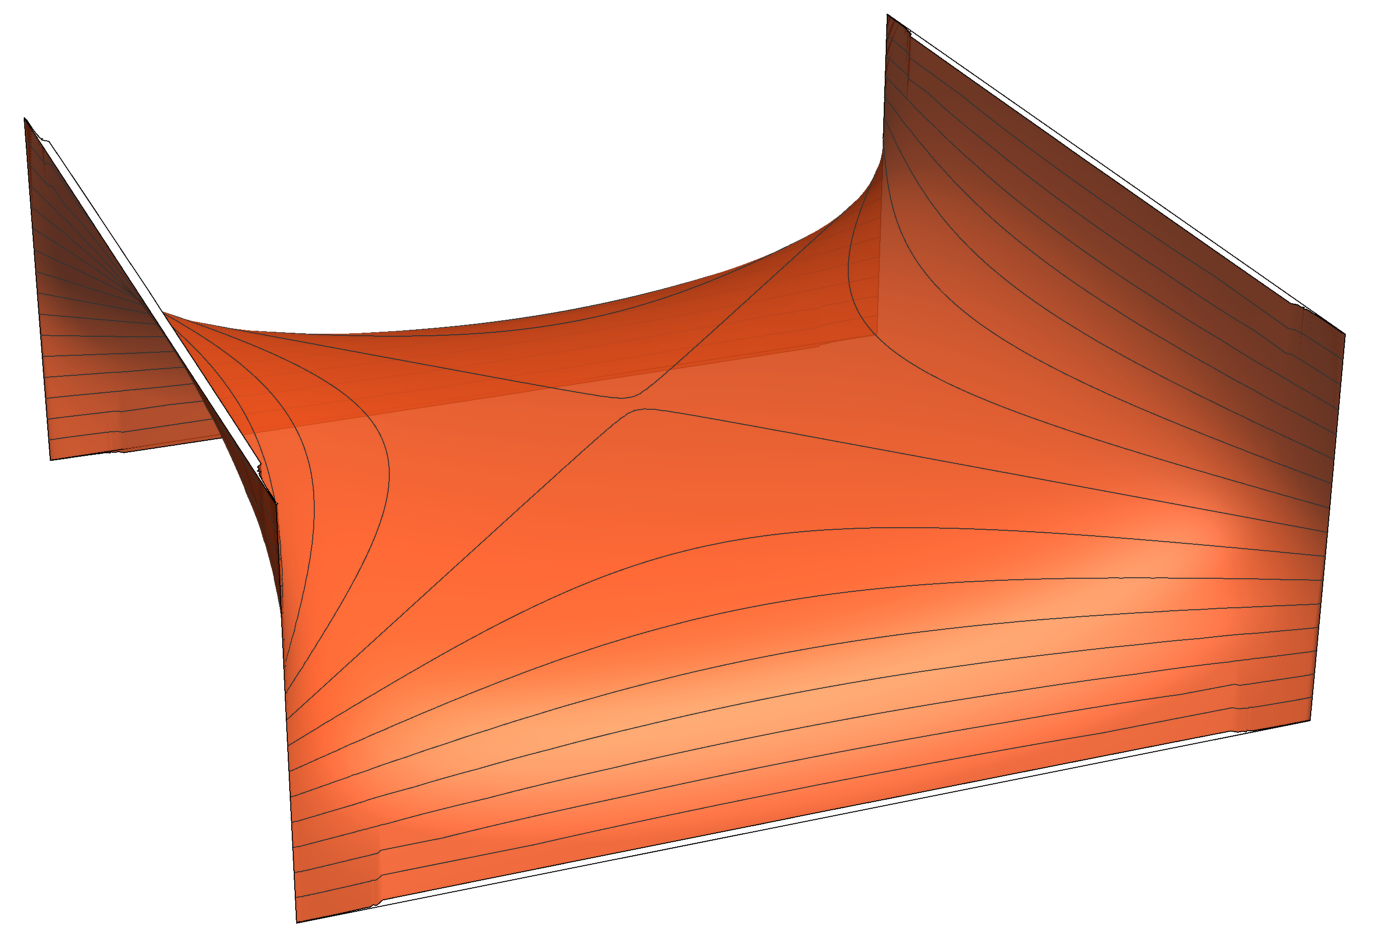
\includegraphics[scale=0.2]{minimal/HFSherk.png}
  \caption{Sattelfläche von Scherk} 
\end{figure}
Die Paare fließen auf der Höhe Null ($z=0$) ineinander. Die dabei gebildete Sattelfläche wird mittels Variationsproblem minimiert, hat gemäß Definition eine Mittlere Krümmung $M=0$. Geometrisch bedingt wiederholt sich die Sattelfläche in $x$ und $y$-Richtung.
\begin{figure}[H]
  \centering
  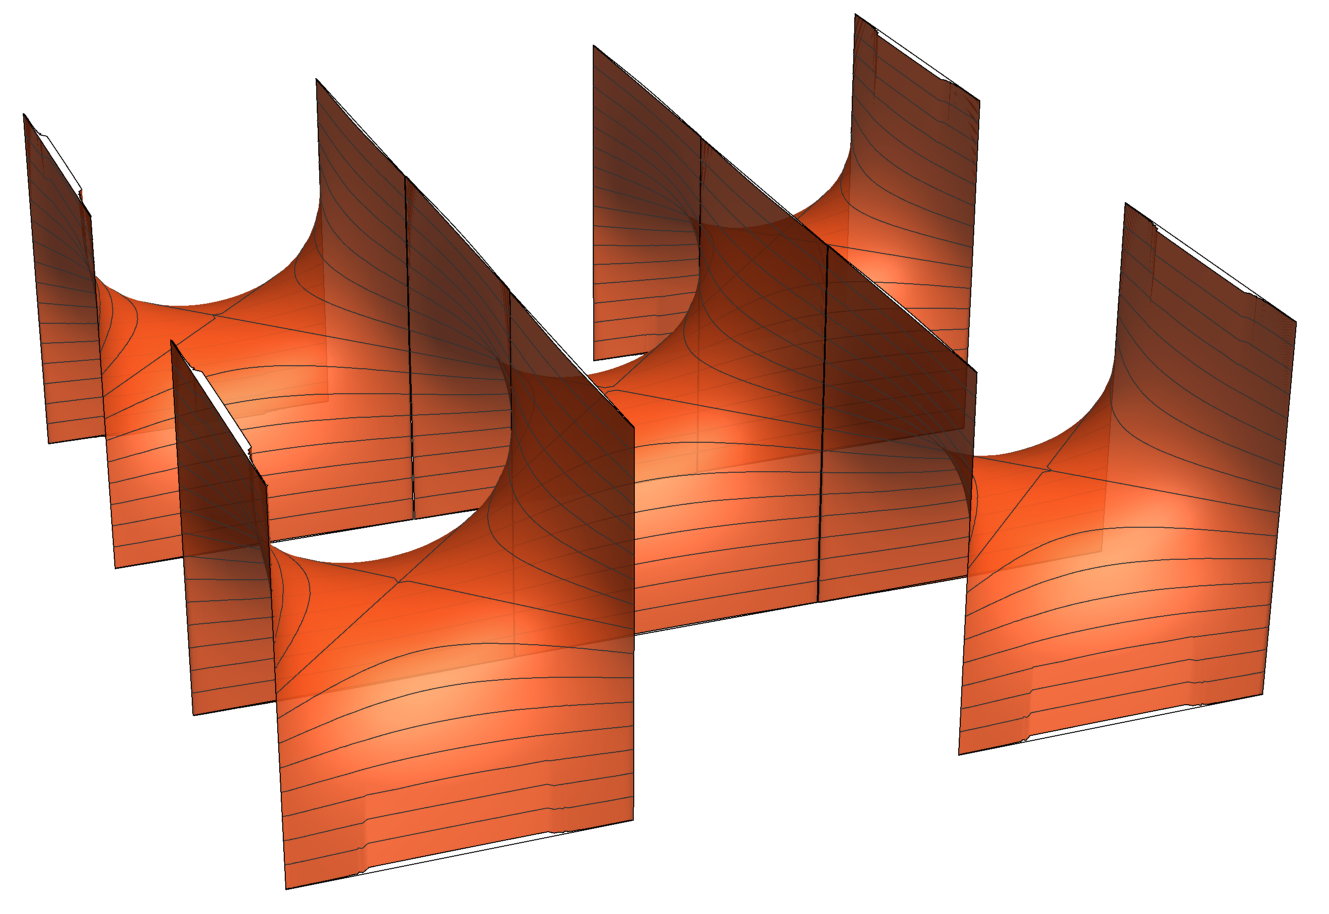
\includegraphics[scale=0.2]{minimal/HFSherk2.png}
  \caption{Neun Perioden der Sattelfläche} 
\end{figure}
Gemäß Definition nach Variationsproblem ist dabei die Mittlere Krümmung $M=0$. Dies wird im Abschnitt \ref{Scherk Herleitung}  nachgerechnet.\\ Eine Approximation an die Fläche kann mittels Drahtgeflecht und einer Seifenlösung nachgebildet werden. Dies folgt direkt aus der äquivalenten Definition \ref{Seifenfilm}. (Photo)
Die Sattelfläche wurde erstmals 1834 von Prof. H. F. Scherk beschrieben und hergeleitet. Sie war nach der in 1776 von Meusnier beschriebene Katenoide die erste neue Minimalfläche. 
\subparagraph{Herleitung}\label{Scherk Herleitung}
Unter Verwendung der Minimalflächengleichung (Referenz)
\begin{equation}\label{Minimalflaechengleichung}
(1+ Z_v^{2})Z_{uu} - 2 Z_u Z_v Z_{uv} + (1+ Z_u^{2}) Z_{vv}=0
\end{equation}
wird nach Lösungen des einfachen Problems $z=Z(u,v)=f(u)+g(v)$ unter den Nebenbedingungen $Z(0,0)=0,\ \nabla Z(0,0)=0$ gesucht. 
Da $ Z_u = f'(u),\ Z_v = g'(v),\ Z_{uu}=f''(u),\ Z_{vv} = g''(v) \ \text{und} \ Z_{uv}=0$ ist, vereinfacht sich die MFG zu 
\begin{equation}\label{MFG Scherk}
(1+g'(v)^2)f''(u)+(1+f'(u)^2)g''(v)=0
\end{equation}
Durch Separieren von $f$ und $g$ stellt sich die Gleichung folglich auf
\begin{equation}\label{MFG Scherk2}
-\dfrac{f''(u)}{1+(f'(u))^2}=\dfrac{g''(v)}{1+(g'(v))^2}=c
\end{equation}
mit $c \in \mathbf{R}$.
Beide Differentialgleichungen werden mittels Separation aufgelöst:
\begin{equation}\label{ScherkDGL1}
\begin{split}
\int -\dfrac{v'(u)}{1+v(u)^2} du &= \int c \ du , \quad v(u)=f'(u) \\
-arctan(v(u)) &= cu+k_1 \\
v(u) &= -tan(cu+k_1)
\end{split}
\end{equation}
Nach der Rücksubstitution wird auf beiden Seiten Integriert:
\begin{equation}\label{SchreckDGL2}
\int f'(u)\ du = \int -tan(cu+k_1)\ du\\
f(u) = \dfrac{log(cos(cu+k_1))}{c}+k_2\\
\end{equation}
mit $f(0)=0$ und $f'(0)=0$ ergibt sich
\begin{equation}
f(u) = \dfrac{log(cos(cu))}{c}\\
\end{equation}
Äquivalent dazu ergibt sich für die 2. DGL:
\begin{equation}
g(v) = - \dfrac{log(cos(cv))}{c}
\end{equation}
Somit lautet die Funktion der Fläche
\begin{equation}
Z(u,v)=\dfrac{log(cos(cu))}{c}-\dfrac{log(cos(cv))}{c}
\end{equation}

\subsection{Young–Laplace - Oberflächenspannung}\label{Young-Laplace}
\subparagraph{Beschreibung}\label{YL-Beschreibung}
Quelle: Landau, L.D. and Lifshitz, E.M.: Fluid Mechanics, Pergamon Press, Oxford
(1987) 
Derivation of the Laplace equation
Svein M. Skjæveland
October 19, 2012
\subparagraph{Herleitung}\label{YL-Herleitung}
Angenommen zwei Medien (z.B. Luft/Wasser) werden durch eine Oberfläche getrennt. Da in den Medien verschiedene Drücke $p_1$ und $p_2$ herrschen, verändert sich die Wölbung der Fläche. Die Veränderung sei $\delta \zeta$. Das Volumen eines einzelnen infinitesimalem Volumensegments sei $\delta \zeta dA$. Dann ist die benötigte Kraft um das Volumensegment um $\delta\zeta$ zu verschieben:
\begin{equation}
\int(-p_1+p_2)\delta \zeta dA
\end{equation}
Die Gesamte Arbeit ergibt sich wenn zur Arbeit der Volumenänderung die Arbeit der Veränderung der Oberfläche $\delta W=\gamma \delta A $ dazu addiert wird, wobei $\gamma$ die Oberflächenspannung und $\delta A$ die veränderte Oberfläche ist. Wir erhalten:
\begin{equation}\label{YL-Arbeit_1}
\delta W=\int(-p_1+p_2)\delta\zeta dA + \gamma\delta A
\end{equation}
Sind $R_1$ und $R_2$ die Radien der Krümmungen der Oberfläche werden die infinitesimale Längenstücke $dl_1$ und $dl_2$ mit $(\delta\zeta /R_1)dl_1$ bzw. $(\delta\zeta /R_2)dl_1$ verlängert. Das Flächenstück $dA=dl_1 dl_2$ verändert sich wie folgt:
\begin{equation}
\begin{split}
dA &= (1+\delta\zeta/R_1)dl_1 (1+\delta\zeta/R_2)dl_2 \\
&\approx dl_1 dl_2 (1+\delta\zeta/R_1 + \delta\zeta/R_2 \\
&\approx dl_1 dl_2 \delta\zeta (\frac{1}{R_1}+\frac{1}{R_2})
\end{split}
\end{equation} 
\begin{figure}[H]
  \centering
  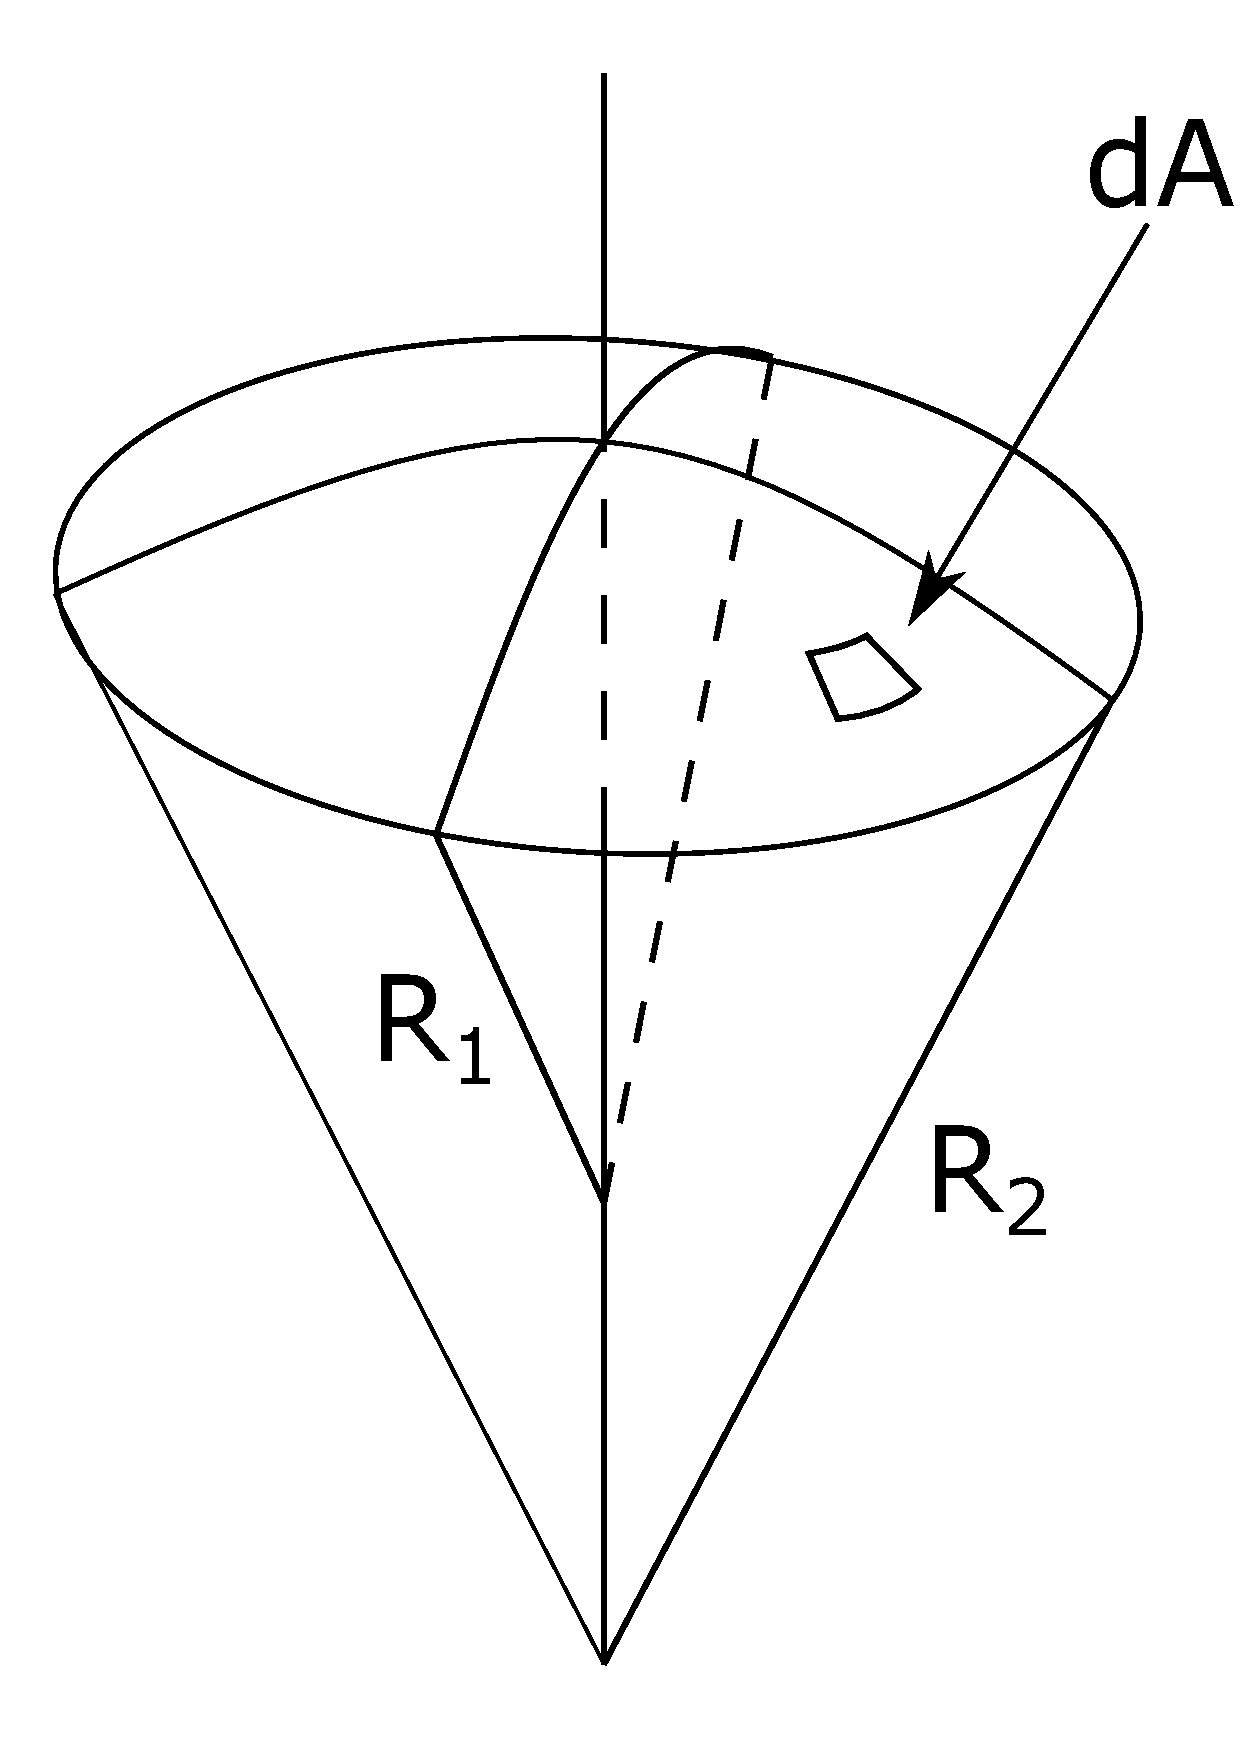
\includegraphics[scale=0.2]{minimal/Young.pdf}
  \caption{Oberflächenspannung} 
\end{figure}
Die veränderte Oberfläche kann damit berechnet und in die Gleichung \ref{YL-Arbeit_1} eingesetzt werden. Befindet sich die Oberfläche im Gleichgewicht muss auch die Veränderung der Arbeit gleich Null sein.
\begin{equation}
\begin{split}
\delta A &= \int \delta\zeta \bigg( \frac{1}{R_1}+\frac{1}{R_2} \bigg) \\
\delta W &= \int \delta\zeta \bigg[ (-p_1+p_2)-\gamma \bigg( \frac{1}{R_1}+\frac{1}{R_2} \bigg) \bigg] =0
\end{split}
\end{equation}
Dies gilt auch für jede Veränderung von $\delta\zeta$. Daraus folgt die finale Formel:
\begin{equation}
-p_1+p_2 = \gamma\bigg( \frac{1}{R_1}+\frac{1}{R_2} \bigg)
\end{equation}
oder
\begin{equation}\label{Young-Laplace}
\Delta p = \gamma\bigg( \frac{1}{R_1}+\frac{1}{R_2} \bigg)
\end{equation}




\subsection{Young–Laplace - Oberflächenspannung}
\printbibliography[heading=subbibliography]
\end{refsection}